
\label{sec:theory}
\def\kt{\ensuremath{k_t}}
\newcommand{\Pmax}{p}
\newcommand{\CCFM}{CCFMa,CCFMb,Catani:1989sg,CCFMd}

The main features of the QCD theory are the confinement
(at short ranges the quarks are strongly bound inside protons)
and the asymptotic freedom (at large scales the coupling constant 
of strong force decreases and quarks become quasi-free partons).
The factorisation theorem exploits these features by 
separating the short and long distances processes, such that 
structure functions can be written as a convolution 
between calculable parts (hard scattering coefficients) and 
non-calculable parts parton distribution functions (PDFs), 
which are therefore parametrised and determined from data.

Factorisation is most rigorously established for deep inelastic 
lepton-hadron scattering. For hadronic processes 
in which a colorless electroweak final state is produced (i.e. Higgs,
 a real or virtual $W$, $Z$ or~$\gamma$) factorisation is also well established
and differential cross section calculations are currently available up to 
next-to-next-to leading order (NNLO) in perturbation theory.

Factorisation is also proved to work for
sufficiently inclusive colored final
states, such as the one-jet and dijet cross section.
In this case no fully rigorous all-order argument is 
available, but no counterexample to factorisation has been found so far.

For the diffractive case, two factorisations are used here: the Regge factorisation
and the collinear factorisation for the hard scattering. 

The proton PDFs are classically extracted from the QCD fits by a measure of 
agreement between data and theory models.
The fit procedure used in \fitter\ framework is common to all the processes and it consists first 
in parametrising PDFs at a starting scale  $Q^2_0$, chosen to be below the charm mass threshold. 
The PDFs are then evolved using coupled, integro-differential
Dokshitzer-Gribov-Lipatov-Altarelli-Parisi (DGLAP)~\cite{Gribov:1972ri,Gribov:1972rt,Lipatov:1974qm,
Dokshitzer:1977sg,Altarelli:1977zs} evolution equations 
as implemented in the QCDNUM~\cite{qcdnum} program, 
at NLO~\cite{Curci:1980uw,Furmanski:1980cm} in the 
$\overline{\text{MS}}$ scheme
%The renormalisation and factorisation scales are set to $Q^2$. 
(LO and NNLO evolutions are also available).
The PDFs calculated at a scale corresponding to an measured cross section are convoluted with the partonic 
cross sections to calculate the predicted cross section. For all measurement points, the predicted 
and measured cross sections together with the corresponding errors are used to build a global $\chi^2$, 
which is minimized to deduce the initial PDF parameters. This generic procedure includes a number of 
subtitles and assumptions, depending on the measurements, scale and available calculations.

In the following sections, the theoretical input for various processes is described,
such as electron-proton deep inelastic scattering (DIS) process in section 
\ref{dis}, $pp$ Drell-Yan process in section \ref{DY}. 
For the jet cross sections calculations, \fitter\ uses  
APPLGRID or FastNLO such as in section \ref{sec:theory:jets}.
In section \ref{ttbar} the $t\bar{t}$ cross sections are calculated based on the HATHOR package.
Alternative approaches to collinear factorisation
are also discussed, see sections \ref{dipole} for Dipole models and 
\ref{TMD} for unintegrated PDFs.
The diffractive PDFs are discussed as well in section \ref{diff}, i.e. PDFs
in the context of the resolved Pomeron model to predict
such processes as seminclusive diffractive scattering in DIS.

%%%%%%%%%%%
\subsection{Deep Inelastic Scattering Formalism and Schemes}
%There are different approaches to the treatment of the heavy quark production. 
%These include the fixed-flavour (FFN) and variable flavour number (VFN) schemes.
%%%%
\label{dis}

The DIS experiments provide the cleanest approach 
to measure the proton structure. 
The DIS experiments are carried either on fixed targets 
or at the collider facilities using electrons, muons or neutrinos 
to probe the proton. 
In the DIS process a lepton is scattered off the constituents of 
the proton by a virtual exchange of neutral (NC) or charged (CC)
 boson producing a hadronic shower and a scattered lepton in the
final state. The schematic of the DIS kinematical variables is illustrated 
in Figure~\ref{fig:dis}:
the negative squared four-momentum of the exchange boson, $Q^2$, the 
scaling variable $x$, which can be related in the parton model to 
the fraction of momentum carried by the struck quark, and the 
inelasticity parameter $y$, which is the fraction of the energy 
transferred to the hadronic vertex. 
\begin{figure}
\begin{center}
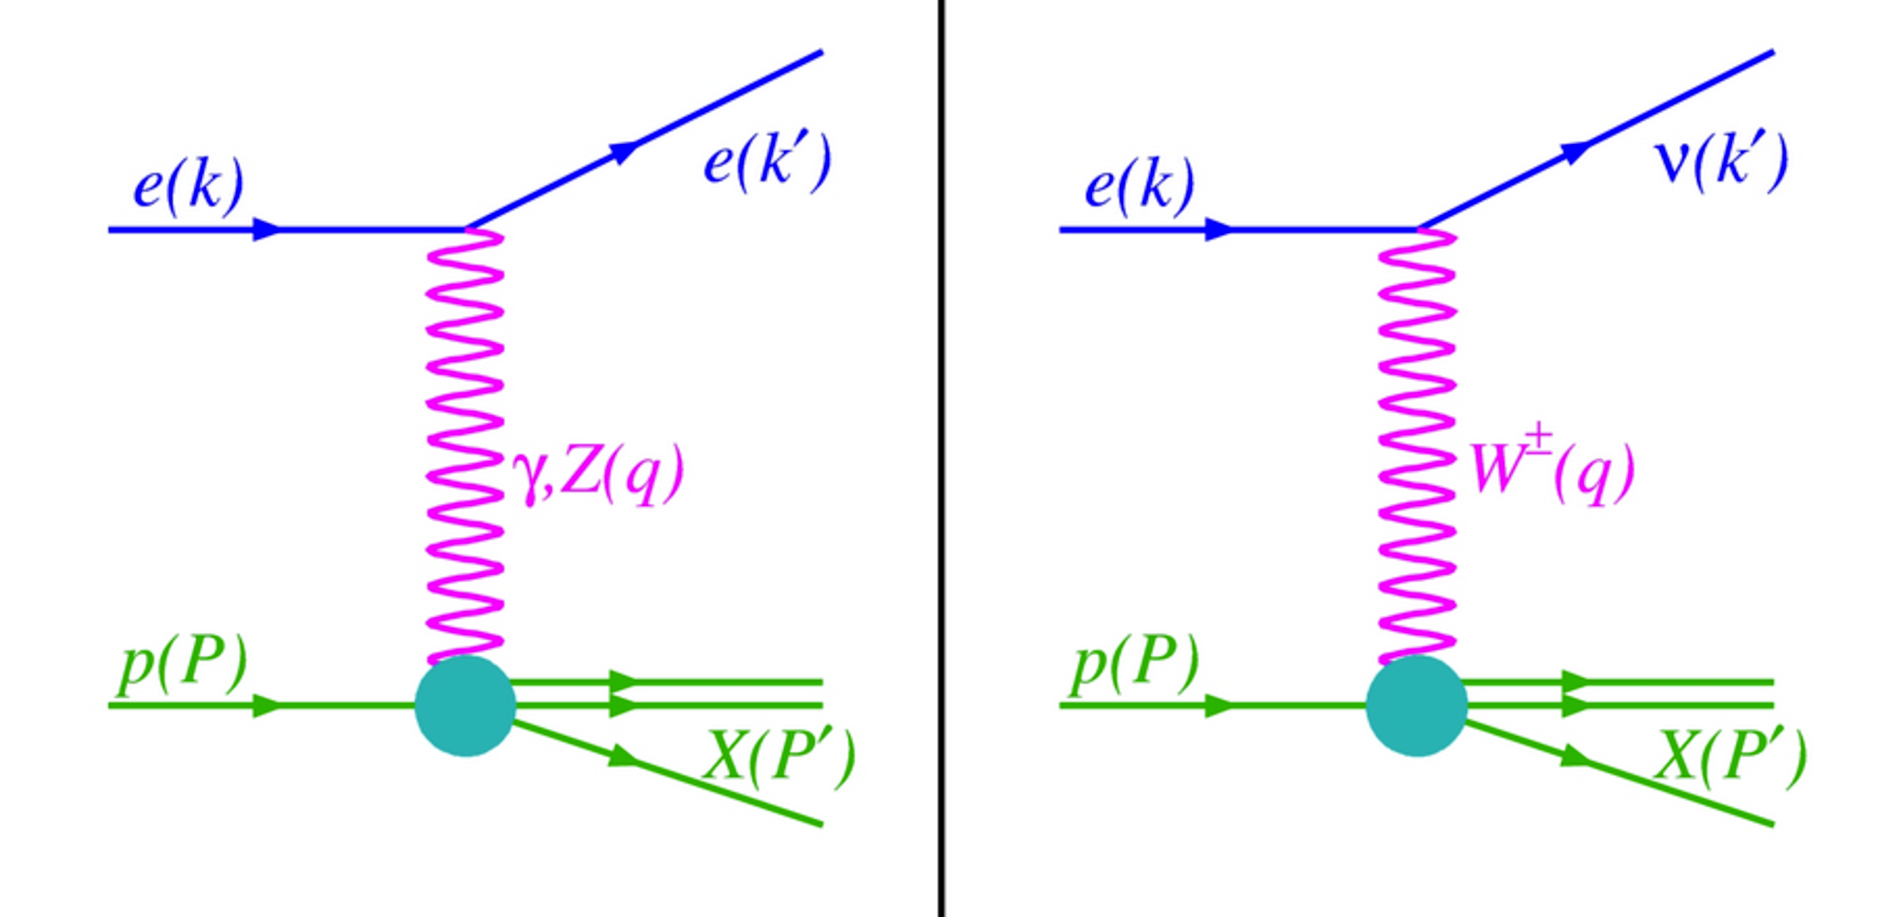
\includegraphics[width=0.5\linewidth]{figures/DIS.pdf}
\end{center}
\caption{Diagram for a neutral and charged current DIS scattering.}
\label{fig:dis}
\end{figure}
%
The NC (and similarly CC) cross section can be expressed in terms of generalised structure functions:
\begin{eqnarray}
   \frac{d^2\sigma_{NC}^{e^{\pm} p}}{dxdQ^2}=\frac{2\pi\alpha^2}{xQ^4} 
    \big [ Y_{+} \tilde F_2^{\pm} \mp Y_{-}x \tilde F_3^{\pm} - y^2 \tilde F_L^{\pm} \big ],
    %\label{eq:NC not reduced}
\end{eqnarray}
where $Y_{\pm} = 1 \pm (1-y)^2$ with $y$ being the inelasticity. The structure function $\tilde F_2$
is the dominant contribution to the cross section, $x \tilde F_3$ is important at high $Q^2$ and $\tilde F_L$ is sizable
only at high $y$.
$\tilde F_2^{\pm}$ and $\tilde F_3^{\pm}$ can be expressed in terms of five structure
functions describing the contributions from pure photon exchange, $\gamma Z$ interference
and pure $Z$ exchange:  
% ------ F_2 ------------
\begin{center}
  \begin{eqnarray}
  \tilde F_2^{\pm} = F_2-v_e \Bigg( \frac{\kappa_W Q^2}{Q^2+M^2_Z} \Bigg)F_2^{\gamma Z}
   + (v_e^2 + a_e^2) \Bigg( \frac{\kappa_W Q^2}{Q^2+M^2_Z} \Bigg)^2 F_2^Z  \\ 
% ------ xF_3 ------------
  x\tilde F_3^{\pm} = \pm a_e \Bigg( \frac{\kappa_W Q^2}{Q^2+M^2_Z} \Bigg)xF_3^{\gamma Z}
  \mp 2a_e v_e \Bigg( \frac{\kappa_W Q^2}{Q^2+M^2_Z} \Bigg)^2 xF_3^Z   
 \end{eqnarray}
\end{center}
Here, the pure photon exchange is described by $F_2$, pure $Z$ exchange by $F_2^Z$ and
$xF_3^Z$, and $\gamma Z$ interference by $F_2^{\gamma Z}$ and $xF_3^{\gamma Z}$.
$v_e$ is the weak vector and $a_e$ the weak axial-vector coupling of the electron
to the $Z$. 
The Weinberg angle $\theta_W$ enters the quantity $\kappa_W$ in the following way: $\kappa_W = \frac{1}{4 \sin^2 \theta_W \cos^2 \theta_W}$.
\\ \\
%
In the framework of perturbative QCD the structure functions are directly related to the
parton distribution functions, i.e. in leading order (LO)  $F_2$ is the momentum sum of quark and anti-quark distributions:
\begin{center}
  \begin{eqnarray}
    \lbrack F_2,F_2^{\gamma Z},F_2^Z \rbrack =
   x \sum_q[e_q^2,2e_qv_q,v_q^2+a_q^2] \{ q(x,Q^2) + \overline q(x,Q^2) \} \\ 
   \lbrack xF_3^{\gamma Z},xF_3^Z \rbrack = 
   x \sum_q[e_q^2a_q,2v_qa_q]\{q(x,Q^2) - \overline q(x,Q^2)\}
 \end{eqnarray}
\end{center}
%$F_2 \approx x \sum e^2_q (q+ \overline q)$, and $xF_3$ is related to their difference,
%$xF_3 \approx x \sum 2e_q a_q (q- \overline q)$. At higher orders, terms related to the gluon density distribution
%($\alpha_s g$) appear.
%\\
In analogy to neutral currents, the inclusive CC $ep$ cross section can be expressed
in terms of structure functions:
\begin{center}
  \begin{equation}
   \frac{d^2\sigma_{CC}^{e^{\pm} p}}{dxdQ^2}=
   \frac{G_F^2}{4\pi x} \bigg( \frac{M_W^2}{Q^2+M_W^2} \bigg)^2
             \big [ Y_{+} W_2^{\pm} + y^2  W_L^{\pm} \mp Y_-x  W_3^{\pm} \big ],
  \label{eq:CC not reduced}
 \end{equation}
\end{center}
Here, $G_F$ is the Fermi constant which is related to the weak coupling $g$ and
electromagnetic coupling $e$, i.e. $G_F = \frac{g^2}{4 \sqrt{2} M_W^2}$.
%
In LO the $e^+p$ and $e^-p$ cross sections are sensitive to different quark
densities:
\begin{eqnarray}
  \begin{array}{rll}
    \tilde \sigma_{CC}^{e^{+} p} = 
    x[\overline u +\overline c] + (1-y)^2 x[ d+s ]  \\
    \tilde \sigma_{CC}^{e^{-} p} = 
    x[ u +c] + (1-y)^2 x[\overline d +\overline s ].
  \end{array}
\end{eqnarray}

The cross-section predictions are obtain by convoluting the PDFs with the 
hard scattering coefficient functions. 
There are various approaches of dividing the structure functions 
into calculable processes and PDFs.
For the DIS processes, those are calculated using the Fixed-Flavour number 
(FFN)~\cite{Laenen:1992, Laenen:1993, Riem:1995} or the general mass 
Variable-Flavour number (GMVFN)~\cite{VFN} schemes. 
%\fitter\ implements the zero mass variable flavour number (ZMVFN) scheme
% from QCDNUM and are discussed in the following subsections.
In the FFN scheme, heavy quark contributions are explicitly included in the hard cross sections. 
In the VFN scheme, PDFs corresponding to heavy quarks are introduced and the number of active 
flavors changes by one unit when the scale crosses the threshold for heavy quark distribution ($Q^2 \ge m_{Q}^2$).


%The various treatments for the heavy quark thresholds are implemented as provided by the MSTW group
The evolution program QCDNUM~\cite{qcdnum} used in \fitter\ provides 
the calculation of the deep inelastic structure functions in the zero-mass, 
generalised mass and the fixed flavour number schemes. 
The VFN schemes with various treatments for the heavy 
quark  thresholds are considered in \fitter\ :
\begin{center}
 \begin{enumerate}
  \item[$\bullet$] the Thorne Roberts (TR) scheme with its variants at NLO and
  NNLO~\cite{Thorne:1997ga,Thorne:2006qt} as provided by the MSTW group,
  \item[$\bullet$] the ACOT scheme with its variants at LO and NLO as provided by the CTEQ group, 
  \item[$\bullet$]  BMSN scheme at NLO and NNLO~\footnote{The BMSN scheme as provided by ABM group
      currently is not yet fully implemented in \fitter\ .}.
  \end{enumerate}
\end{center}  
The fixed-flavour number scheme
is available via the QCDNUM implementation and via the 
{\tt OPENQCDRAD}~\cite{openqcdrad:page} interface.
Each of these schemes is briefly discussed in further details.


\subsubsection{Zero-Mass Variable Flavour Scheme}

In the zero-mass variable flavour number scheme (ZM-VFNS) heavy quark densities are
included in the proton for $Q^2>>m_h^2$ but they are treated as massless in both,
the initial and final states.
This scheme is accurate in the region where $Q^2$ is much greater than $m_h^2$
but becomes unreliable for $Q^2 \sim m_h^2$. 

%The un-polarised DIS structure functions in ZM-VFN scheme are computed as a 
%convolution of the parton densities with zero-mass coefficient functions and 
%in \fitter\ are activated via namelist {\tt HF$\_$SCHEME} in the {\tt steering.txt}.
%%%%
\subsubsection{General Mass Variable Flavour Scheme: Thorne-Roberts scheme}

The Thorne-Roberts (TR) scheme, (refered as RT scheme in the \fitter\ )
is a general-mass variable flavour number scheme (GM-VFNS)
 used as default for the MTSW PDF sets. GM-VFNS smoothly connects the two regions: 
scales below the heavy quark mass scale ($Q^2<m_h^2$) and scales much above the heavy quark scale threshold ($Q^2>>m_h^2$). However, the definition is not unique.
A GM-VFNS can be defined by demanding equivalence of the $n_f = n$ (FFNS) and $n_f = n+1$ flavour (ZM-VFNS) descriptions above the transition point for the new parton distributions
(they are by definition identical below this point), at all orders.

The TR scheme has two different variants depending on the treatment across the threshold of heavy quarks: TR standard (as used in MSTW PDF 
sets~\cite{Thorne:2006qt,Martin:epC63}) 
and TR optimal~\cite{Thorne:6180}, with a smoother transition across the heavy quark mass scales. Both of these variants are accessible within the \fitter\ package.
The calculations are available to NLO and NNLO order. In addition, a fast version of the scheme is available (i.e. RT FAST) by using the k-factor technique. 
The k-factors are applied at the first iteration of the minimisation process enabling the code to run fast, as the k-factors are defined as the ratio between massless and massive scheme, while the massless scheme accessed via QCDNUM is very fast.

 
%%%%
\subsubsection{General Mass Variable Flavour Scheme: ACOT scheme}

The Aivazis-Collins-Olness-Tung scheme belongs to the group of VFN 
factorisation schemes that use the renormalization method of 
Collins-Wilczek-Zee (CWZ) \cite{CWZ}.
This scheme involves a mixture of the $\overline{\text{MS}}$ scheme 
for light partons (and for heavy partons when the factorisation scale 
is larger than the heavy quark mass) and the zero-momentum subtraction 
renormalisation scheme for graphs with heavy quark lines 
(if factorisation scale is smaller than the mass of the heavy quark threshold). 
The DGLAP kernels and PDF evolution are pure  $\overline{\text{MS}}$.
 Definition of subtractions is analogous to  $\overline{\text{MS}}$. 
Therefore, the ACOT scheme is considered to be a minimal extension of $\overline{\text{MS}}$ scheme.


Within the ACOT package, different variants of the ACOT scheme are available:
ACOT Full, ACOT-S, ACOT
Chi,  $\overline{\text{MS}}$  at LO and NLO. 
For the longitudinal structure function higher order
 calculations are also available. 
The ACOT Full implementation fully takes into account the quark masses and it reduces
to  $\overline{\text{MS}}$  in the limit of masses going to zero, but it has the disadvantage 
of being quite slow.
Therefore the k-factor technique has been addopted within the \fitter\  
machinery to be able to perform QCD fits. The k-factor can be defined in two different ways:
on one hand as the ratio between same order calculations but massless vs massive 
(i.e. NLO (ZMVFNS)/NLO (ACOT), on the other hand one could speed up the calculations by 
defining the k-factors as the ratio between LO (massless)/NLO (massive).
Both options are available in the \fitter\ package and give similar results. 
%k-factors depend on PDFs therefore same iterations of the fit are needed.
For convergence of the k-factors usually $2-3$ iterations are needed.
These different variants of this scheme are all integrated in the \fitter\  framework and can be 
selected via namelist {\tt HF$\_$SCHEME} in the {\tt steering.txt} (ACOT ZM, ACOT FULL, ACOT CHI, ACOT-S).



The differences between TR and ACOT scheme types are nicely summarised in the figure \ref{fig:schemes}.
One major issue in a complete GM-VFNS, is that of the ordering of the
perturbative expansion.
 The equivalency of swapping the $O(m_{H}^2/Q^2)$ 
terms without violating the definition of a GM-VFNS is what mainly distinguish the ACOT from TR schemes. 

\begin{figure}
\begin{center}
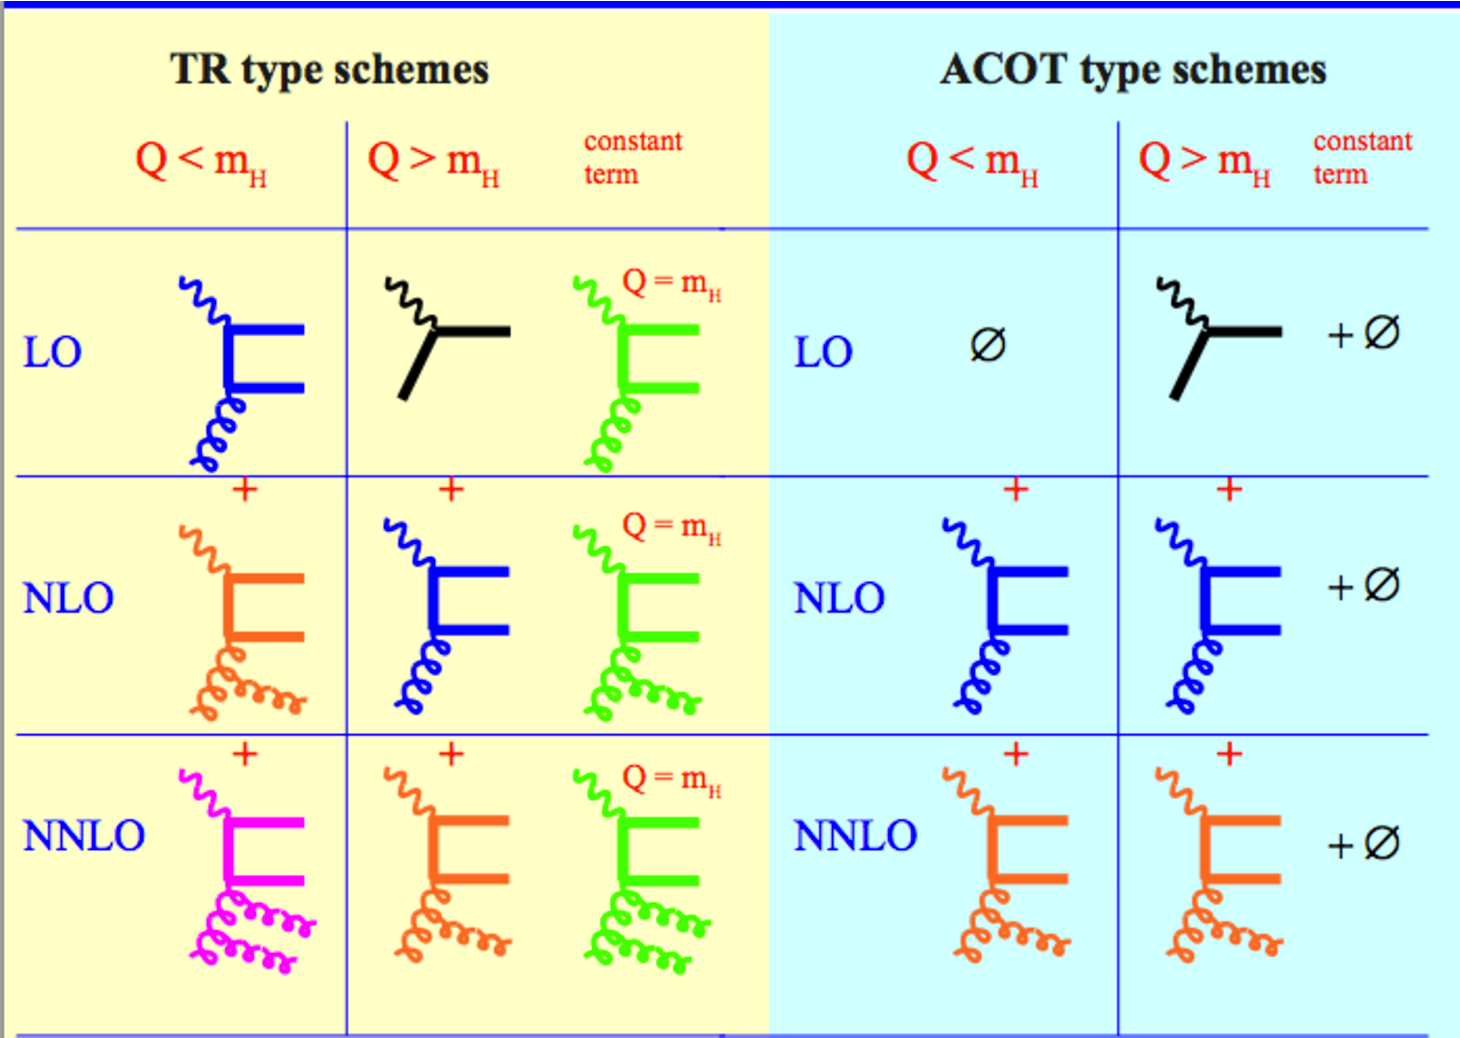
\includegraphics[width=0.5\linewidth]{figures/schemes.pdf}
\caption{Schematic Summary of ACOT  and TR  Schemes}
\label{fig:schemes}
\end{center}
\end{figure}


%%%%
\subsubsection{Fixed -Flavour Number Scheme}

The fixed-flavour number scheme for DIS structure functions in \fitter\ can be selected via {\tt HF$\_$SCHEME}
using QCDNUM or ABM~\cite{openqcdrad:page} implementation.
As mentioned before, in the FFN scheme only gluon and the light quarks are considered
as partons within the proton, massive quarks are produced perturbatively in the final state.

In addition, the recent variant of the fixed-flavour number scheme in which the running mass definition 
is used in the $\overline{\text{MS}}$ scheme~\cite{Alekhin:runm} can be selected
in \fitter\ .This variant is realised via the interface to the open-source code 
OPENQCDRAD~\cite{openqcdrad:page}.
This scheme has the advantage of reducing the sensitivity of the DIS cross sections to
higher order corrections, and improving the theoretical precision of the mass definition. 
\\           
In QCDNUM, the calculation of the heavy quark contributions to DIS structure functions
are available at NLO and only electromagnetic exchange contributions are taken into account.
In the ABM implementation, the QCD corrections to the massive Wilson coefficients 
up to the NNLO for the neutral-current (NC) heavy-quark production~\cite{SMoch} and up to NLO
for the charged-current (CC) case are available.
%
%The fixed-flavour number scheme for  in \fitter\ can be also accessed via interface to
%the open-source code OPENQCDRAD~\cite{openqcdrad:page} in \fitter\ framework 
%provides an access to 
%fixed flavour number scheme (FFNS)~\cite{Laenen:1992,Laenen:1993,Riem:1995}
%
%By default, in FFNS the number of light quark 
%flavours $n_{f}$ (here $n_{f}=3$) are considered in the PDF evolution and heavy (massive) 
%quarks appear only in the final state. 
%The QCD corrections to the massive Wilson coefficients which are known up to the NNLO
%for the neutral-current (NC) heavy-quark production~\cite{} are implemented in OPENQCDRAD.
%In the case of charged-current (CC), the massive NLO QCD corrections~\cite{} are available.
%In addition, the treatment of the heavy-quark contributions in DIS are provided 
%in both, the pole-mass and the running-mass definition in $\overline{\text{MS}}$ 
%scheme~\cite{Alekhin:runm}. \\
%In case the FFN scheme is chosen as the fitting option (see corresponding instructions in the section 1),
%the heavy quark contributions to DIS structure functions $F_2$ and $F_L$ (and $F_3$ in the charged 
%current case) are calculated in the FFNS and together with the light-flavor contributions are 
%provided for the theory prediction calculation (theory$\_$dispatcher.f).
%The interpolation to PDFs and $\alpha_s$ evolution from QCDNUM are set up in the interface to OPENQCDRAD. \\
%The variation of the renormalisation and factorisation scales for heavy quarks is 
%possible (see available options in steering.txt file).
%
%       
%%%%%%%%%%%
\subsubsection{\texorpdfstring{$ep$}{ep} Electroweak corrections}
%%%%%%%%%%%
 
To properly compare the experimental data with theoretical predictions, 
QED corrections are necessary. In the \fitter\, the electroweak corrections 
for the DIS process are based on the EPRC package provided by Hubert Spiesberger \cite{HS}.
%The measured cross sections as presented by HERA are not corrected for the weak corrections
%in order to retain sensitivity to higher order EW effects.

The calculations of higher-order electroweak corrections to DIS scattering at HERA are performed
in the on-shell scheme where the gauge bosons masses $M_W$ abd $M_Z$ are treated symmetrically
as basic parameters together with the top and Higgs masses, besides the fine structure constant 
$\alpha$ and other fermion masses.

The code provides the running of $\alpha$ using the most recent parametrisation
of the hadronic contribution to $\Delta_\alpha$ \cite{Jegerlehner}, as well as an older 
one from Burkhard \cite{Burkhard}.
For the Drell Yan processes there are independent treatments applied as $k-factors$ (such as 
from SANC, FEWZ packages).

 


\subsection{Drell Yan processes}
%%%%
\label{DY}

This section presents calculations of Drell Yan processes that can be used to 
predict lepton pair production at the LHC or Tevatron.
A schematic of the Drell Yan process is illustrated in Figure~\ref{fig:dy}.
\begin{figure}
\begin{center}
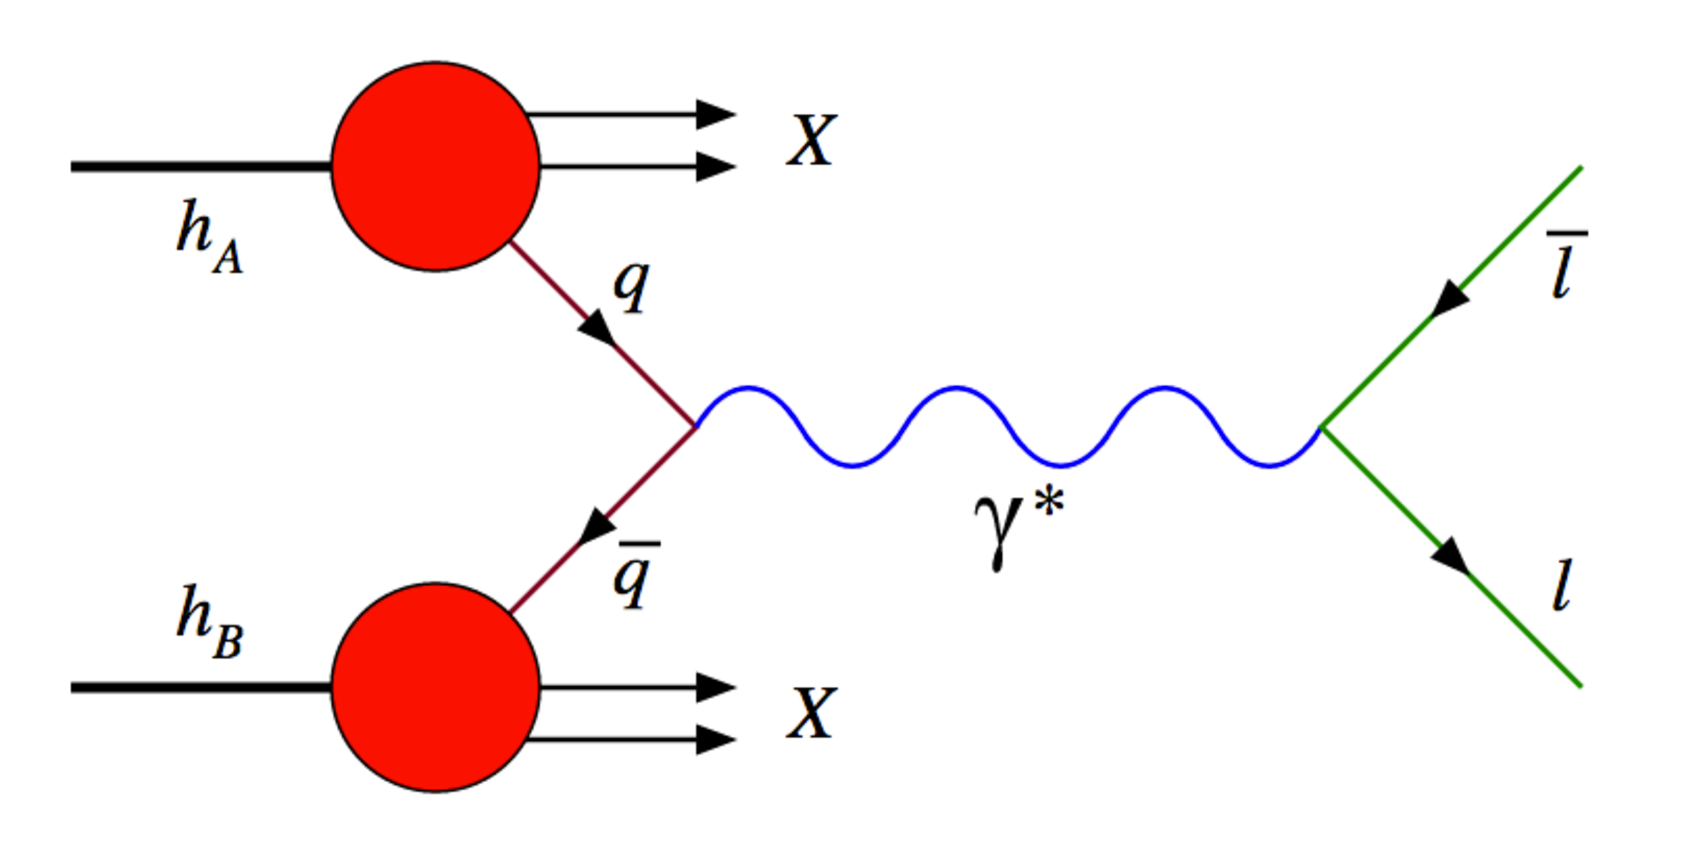
\includegraphics[width=0.5\linewidth]{figures/dy.pdf}
\end{center}
\caption{Diagram for a generic DY scattering.}
\label{fig:dy}
\end{figure}
The calculations of the Drell Yan processes are known for many observables up to  the NNLO order.
 For example, there are packages such as FEWZ~\cite{FEWZ}, DYNNLO~\cite{DYNNLO} for NNLO,
 or MCFM~\cite{MCFM} for NLO calculations. However, due to the complicated nature of these
 calculation involving an increased number of diagrams with additional higher order, these calculations are too slow to be used iteratively in a fit.
There are various methods to overcome this shortage: using the $k-factors$ approximation from lower to higher order,  or using the grid technique when available.
  
 \fitter\ provides two implementations
for $pp$  Drell Yan processes.
 The first implementation uses calculations at LO which can be extended to NLO using k-factors,
the second uses the APPLGRID interface.
For thorough details of the theoretical modules we direct the user to read the provided references of these packages.


The leading order Drell-Yan~\cite{Drell:1970wh,Yamada:1981mw} cross section 
for the neutral current, triple differential in
invariant mass \(M\), boson rapidity \(y\) and CMS
lepton scattering angle \(\cos\theta\), can be written as
\begin{align}
\frac{\mathrm{d}^3\sigma}{\mathrm{d}M\mathrm{d}y\mathrm{d}\cos\theta} &=
  \frac{\pi\alpha^2}{3MS}\sum_{q}P_q
  \left[F_q(x_1,Q^2)F_{\bar{q}}(x_2,Q^2) + (q\leftrightarrow\bar{q})\right],
\end{align}
where \(S\) is the squared CMS beam energy, \(x_{1,2} = \frac{M}{\sqrt{S}}\exp(\pm y)\), $F_q(x_1,Q^2)$ parton distribution functions, and 
\begin{align}
  P_q &=  e_l^2e_q^2(1+\cos^2\theta) \nonumber \\
      &+  e_le_q\frac{2M^2(M^2-M_Z^2)}{\sin^2\theta_W\cos^2\theta_W
          \big[(M^2-M_Z^2)^2+\Gamma_Z^2M_Z^2\big]}
          \big[aA_q(1+\cos^2\theta)+2bB_q\cos\theta\big] \nonumber \\
      &+  \frac{M^4}{\sin^4\theta_W\cos^4\theta_W
          \big[(M^2-M_Z^2)^2+\Gamma_Z^2M_Z^2\big]}
          \big[(a^2+b^2)(A_q^2+B_q^2)(1+\cos^2\theta)+8abA_qB_q\cos\theta\big].
\end{align}
Here \(\theta_W\) is the Weinberg angle, \(M_Z\) and \(\Gamma_Z\) are Z boson mass and 
width, and
\begin{align}
 a & = -\frac{1}{4} + \sin^2\theta_W,  \nonumber \\
 b & = -\frac{1}{4},  \nonumber \\
 A_q & = \frac{1}{2}I_q^3-e_q\sin^2\theta_W, \nonumber \\
 B_q & = \frac{1}{2}I_q^3,  \nonumber \\
 I_u^3 & = -I_d^3 = \frac{1}{2},  \nonumber \\
 e_l & = -1, e_u = \frac{2}{3}, e_d = -\frac{1}{3}.
\end{align}

The expression for charged current has a simpler form:
\begin{align}
\frac{\mathrm{d}^3\sigma}{\mathrm{d}M\mathrm{d}y\mathrm{d}\cos\theta} &=
 \frac{\pi\alpha^2}{48S\sin^4\theta_W}
 \frac{M^3(1-\cos\theta)^2}{(M^2-M_W^2)+\Gamma_W^2M_W^2}
 \sum_{q_1,q_2}V_{q_1q_2}^2F_{q_1}(x_1,Q^2)F_{q_2}(x_2,Q^2),
\end{align}
where \(V_{q_1q_2}\) is the CKM quark mixing matrix and \(M_W\) and \(\Gamma_W\)
are \(W\) boson mass and decay width.

The simple form of these expressions allows to calculate integrated
cross sections without utilization of Monte-Carlo techniques.
This is particularly useful for PDF fitting purposes because
the statistical fluctuations are avoided in this case. In both 
neutral and charge current expressions the parton density functions
factorise as a function dependent only on boson rapidity \(y\) and
invariant mass \(M\) leaving \(\cos\theta\) dependence aside.
The integral in \(\cos\theta\) can be computed analytically and
integrations in \(y\) and \(M\) can be performed with the Simpson
method. The \(\cos\theta\) parts are kept in the equation 
explicitly because their integration is asymmetric for
data in lepton \(\eta\) bins and also is being performed when applying 
the lepton \(p_{\perp}\) cuts.

The fact that PDF functions factorise,
it allows to significantly boost calculations when 
performing parameter fits over lepton rapidity data. In this case
the factorised part of the expression which is independent on PDFs can be
calculated only once for all minimisation iterations.
The leading order code in \fitter\ package implements this 
optimisation and uses fast convolution routines provided by
QCDNUM. Currently the full width LO calculations are optimised 
for lepton pseudorapidity and boson rapidity distributions with the
possibility to apply lepton \(p_{\perp}\) cuts, making this procedure
flexible to describe data.

The calculated leading order cross sections are multiplied by
NLO or NNLO $k-factors$ provided for corresponding data distributions.
%%%%


On the other hand, one can obtain directly the NLO predictions by using APPLGRID or FASTNLO techniques, which rely on factorisation theorem by decoupling the hard scattering coefficients from PDFs. Therefore, the calculated hard scattering coefficients can be stored into a grid for a given kinematic bin, speeding up the convolution process with the PDFs allowing to be used for QCD fits. 
These method are described in more details in sections \ref{sec:theory:jets}

%%%%%%%%%%%
\subsection{\texorpdfstring{$t\bar{t}$}{t-tbar} Cross Sections via {\tt HATHOR}}
\label{ttbar}
This section presents the calculation tool available 
in \fitter\ for top-guark pair prouction in $p \bar{p}$ and $pp$ collisions.

Top-quark pairs ($t\bar{t}$) are mainly produced at hadron colliders via $gg$ fusion and
$q \bar q$ annihilation. Furthermore, there are the $q q'$ and
$q g$ production modes.
The program HATHOR~\cite{Aliev:2010zk} allows calculating
the expected total $t \bar t$ cross section at 
$p \bar p$ and $p p$ colliders up to approximate NNLO accuracy.
Version 1.3 of HATHOR includes the exact NNLO for $q \bar q \to t \bar t$ \cite{Baernreuther:2012ws}
as well as a new high-energy constraint on the approximate NNLO obtained from
soft-gluon resummation \cite{Moch:2012mk}.
The default choice for renormalization and factorization scale in $t \bar t$ production is the top-quark mass, $m_t$.
The pole mass scheme is typically employed for $m_t$ but HATHOR also supports calculations in
the $\overline{\text{MS}}$ scheme.
\subsection{Jets}
\label{sec:theory:jets}
In this subsection, the use of the factorisation formalism is fully exploited for the 
calculations of the inclusive jets and dijet cross sections.
This sections presents various fast tool techniques based on this concept.


The calculation of higher order jet cross sections is very demanding
in means of computing power. The reasons are the large number of contributing
Feynman diagrams and also the large number of infrared divergencies.
For an accurate cancellation of these singularities, typically, the 
dipole subtraction method is applied in such calculations.
During the necessary Monte Carlo integration a very fine phase
space sampling has to be performed in order to account for the
accurate cancellation of the counter terms.

In order to enable the inclusion of jet-cross section 
measurements in PDF and $\alpha_s$ fits, these perturbative
coefficients have to be pre-computed in a PDF and $\alpha_s$ 
independent way. For this purpose, two quite similar tools are
interfaced to the \fitter .

\subsubsection{FastNLO}
The fastNLO project~\cite{Kluge:2006xs,Wobisch:2011ij,Britzger:2012bs}
enables the inclusion of jet data in PDF and $\alpha_s$ fits.
This tool uses multi-dimensional interpolation
techniques to convert the convolutions of perturbative 
coeffcients with parton distribution functions and 
the strong coupling into simple products.
Although the concept is process independent, the perturbative 
coefficients are usually calculated by the \texttt{NLOJET++}
program~\cite{Nagy:1998bb} where calculations for jet-production
in DIS~\cite{Nagy:2001xb}  as well as in hadron-hadron 
collisions~\cite{Nagy:2003tz,Nagy:2001fj} are available.
Also threshold-corrections of $\mathcal{O}$(NNLO) for 
inclusive jet cross sections in hadron-hadron collisions are
available~\cite{Kidonakis:2000gi}.

The fastNLO libraries are standardized included in the \fitter\
package and no further requirements or compilation options
are needed. In order to include a new measurement into the PDF-fit,
the fastNLO table have to be specified. These tables include all
necessary informations of the perturbative coefficients and the
calculated process for all bins of a certain dataset. 
Tables for almost all published jet measurements
are available through the project website {\tt http://fastnlo.hepforge.org}.
%or have otherwise to be calculated by using the full fastNLO package.

Features of the fastNLO concept are the very quick convolution of the
perturbative coefficients with the PDFs of
$\mathcal{O}(100 ms)$ and the very high accuracy
of the interpolation procedure. 
The fastNLO tables are conventionally calculated
for multiple factors of the factorization scale, 
and the renormalization scale factor can be choosen freely.
Some of the fastNLO tables already involve a scale-independent
concept~\cite{Britzger:2012bs}, which allows for 
the free choice of the renormalization and the factorization
scale as a function of two pre-defined observables.
The evaluation of the strong coupling constant, which enters
the cross section calculation, is taken consistently from the 
QCDNUM evolution code.


\subsubsection{APPLGRID}
The APPLGRID~\cite{Carli:2010rw} package allows to compute a fast estimate
of NLO cross sections for particular processes for arbitrary set of 
proton parton density functions. The package implements
calculations of Drell Yan cross sections of electroweak boson (\(Z,W\))
production as well as jet production in proton-(anti)proton
collisions and DIS processes. 

The approach is based on storing perturbative coefficients
of NLO QCD calculations of final-state observables measured
in hadron colliders in look-up tables. The PDFs and the 
strong couplings are included during the final calculations,
e.g. during the PDF fits procedure. The method allows 
variation of factorization and renormalization scales in
calculations.

The look-up tables (grids) can be generated with modified versions of
of MCFM~\cite{Campbell:1999ah,Campbell:2010ff} or 
NLOjet++~\cite{Nagy:2001fj} software distributed
with the full version of APPLGRID package.
% NLO calculations
%for the current analysis are performed with the help of APPLGRID
%generated grids based on MCFM calculations. 

APPLGRID supports the interface to the MCFM parton level generators,
hence the model input parameters such as electroweak parameters
are in fact pre-set following the MCFM input steering card, while
binning and definitions of the observables for which the
differential cross sections are needed are set in the 
APPLGRID code. 
The grid parameters \(x_1, x_2\) and \(Q^2\) binning
and interpolation orders are also defined in the code.

APPLGRID performs construction of the grid tables in two 
steps: {\it (i)} exploration of the phase space in order
to optimize the memory storage and {\it (ii)} actual grid
construction in the phase space corresponding to the 
requested observables.

Afterwards the NLO cross sections are restored from the grids
with providing PDFs, \(\alpha_S\), factorization and 
renormalization scales and with QCD NNLO $k-factors$ applied
if stated.

%%%%%%%%%%%
\subsection{DIPOLE models}
\label{dipole}
%At low $x$ and low $Q^{2}$, virtual photon-proton scattering is described using the colour
%dipole model formalism~\cite{NNZ:91}. Within this formalism, the scattering process is calculated as a fluctuation of the
%photon into a quark-antiquark pair (dipole), with a lifetime $\propto\enskip 1/x$, which interacts with the proton.
%
%Several approaches have been developed to phenomenologically describe the dipole-proton interaction
%cross section, three of which are implemented in the fitter\. These are
%the original model version (GBW)~\cite{Golec-Biernat:1998js}, a model based on the colour glass condensate approach
%to the high parton density regime (IIM)~\cite{Iancu:2003ge}, and a modified GBW model by adding effects of the 
The dipole picture provides an attractive approach to the virtual photon-proton
 scattering in the low $x$ region because it allows to describe inclusive and 
diffractive processes together.
 In this approach the virtual photon fluctuates into a $q\bar q$ (or $q\bar q g$) 
 dipole which interacts with the proton~\cite{NNZ:91}.  
The dipoles can be viewed as quasi-stable quantum mechanical states, which have very long 
life time $\propto 1/m_p x\;$ and a size which is not changed by scattering.
 A schematic view of dipole factorisation at small x in DIS is illustrated in Figure~\ref{fig:dipole}
The virtual photon fluctuates into a quark-antiquark pair and subsequently interacts with the target, 
and the dynamics of the interaction are embeded in the dipole scattering amplitude.

\begin{figure}
\begin{center}
\caption{Schematic diagram of dipole factorisation for the inclusive cross section in DIS.}
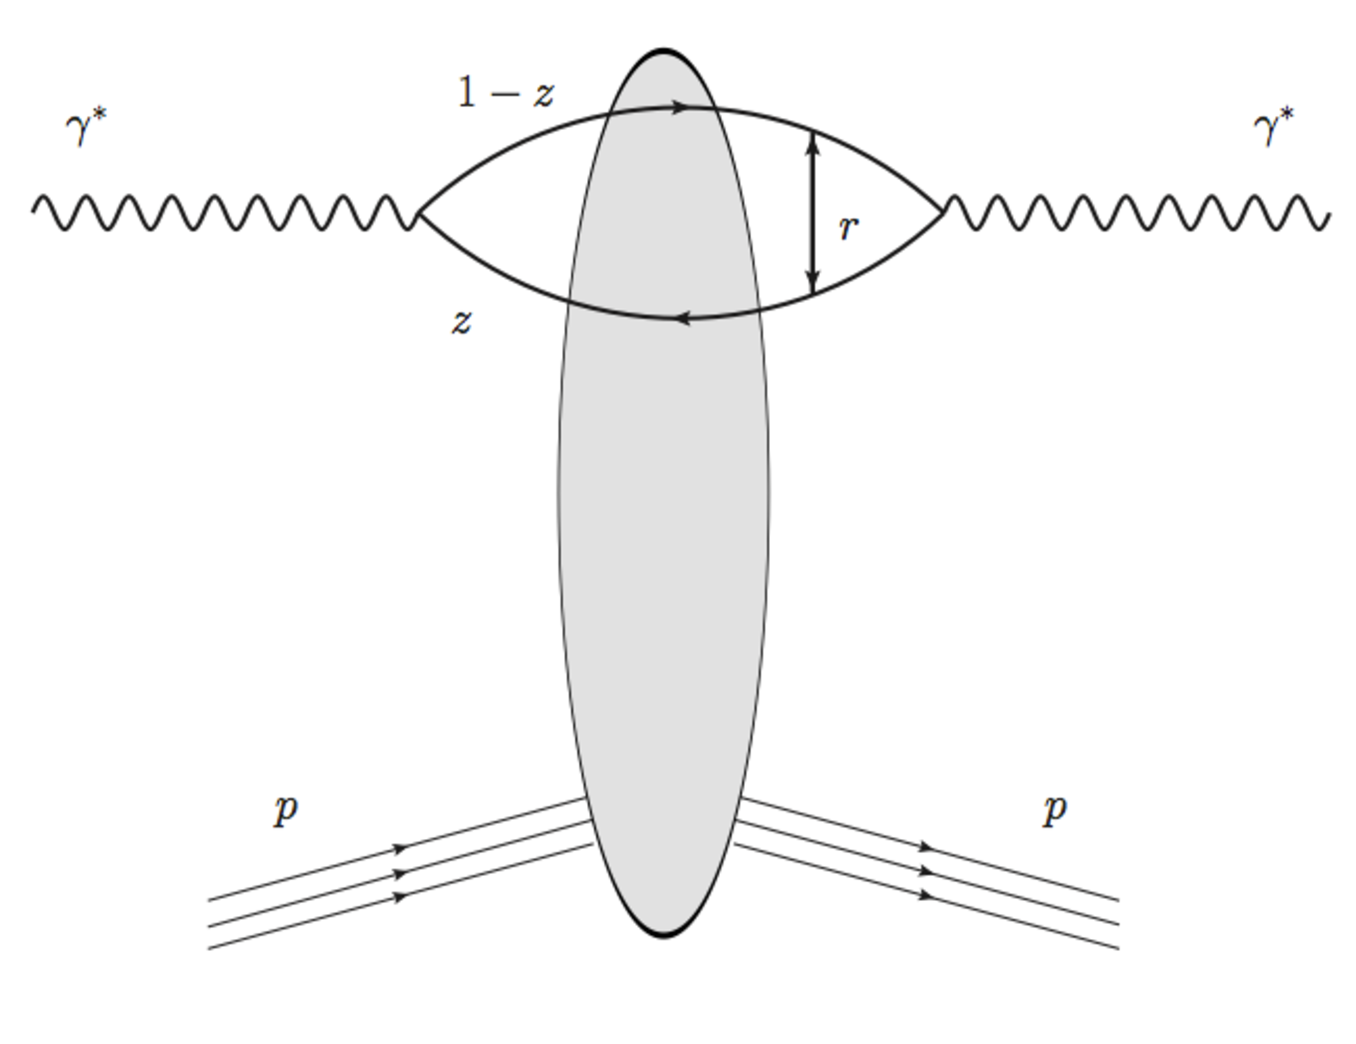
\includegraphics[width=0.5\linewidth]{figures/dipole.pdf}
\end{center}
\label{fig:dipole}
\end{figure}

Several dipole models have been developed to describe various DIS reactions. They vary due to different assumption made about the behavior of the dipole cross sections.   In the \fitter\  three representative models  are implemented:
\begin{itemize}
\item the original Golec-Biernat-W\"usthoff (GBW)~\cite{Golec-Biernat:1998js} 
dipole saturation model,
\item the colour glass condensate approach to the high parton density 
regime Iancu-Itakura-Munier (IIM) model~\cite{Iancu:2003ge},
\item a modified GBW model which takes into account the effects of  
DGLAP evolution Bartels-Golec-Kowalski(BGK)~\cite{Bartels:2002cj}.
\end{itemize}
%%%%
\subsubsection{GBW model}

In the GBW model the dipole-proton cross section $\sigma_{\text{dip}}$ is given by
\begin{equation}
\label{eGBW}
   \sigma_{\text{dip}}(x,r^{2}) = \sigma_{0} \left(1 - \exp \left[-\frac{r^{2}}{4R_{0}^{2}(x)} \right]\right),
\end{equation}
where $r$ corresponds to the transverse separation between the quark and the antiquark, and $R_{0}^{2}$
 is 
%an $x$ dependent scale parameter, having the form $R_{0}^{2}(x)=\left(x/x_{0}\right)^{\lambda}$.
an $x$ dependent scale parameter which has a meaning of saturation radius,  $R_{0}^{2}(x)=\left(x/x_{0}\right)^{\lambda}$.
The free fitted parameters are the cross-section normalisation $\sigma_{0}$ as well as $x_{0}$ and $\lambda$.
%%%%
\subsubsection{IIM model}
The IIM model assumes an improved expression for the dipole cross section which is based on the 
Balitsky-Kovchegov equation~\cite{Balitsky:1995ub}. The explicit formula for $\sigma_{\text{dip}}$ 
can be find in~\cite{Iancu:2003ge}. The free fitted parameters are the alternative scale parameter $\tilde{R}$, $x_{0}$ and $\lambda$.
%%%%
\subsubsection{BGK model}
The BGK model modifies the GBW model by taking into account the  DGLAP evolution
of the gluon density. 
The dipole cross section is given by
\begin{equation*}
\label{eBGK}
   \sigma_{\text{dip}}(x,r^{2}) = \sigma_{0} 
\left(1 - \exp \left[-\frac{\pi^{2} r^{2} \alpha_{s}(\mu^{2}) xg(x,\mu^{2})}{3 \sigma_{0}} \right]\right).
\end{equation*}
The factorization scale $\mu^{2}$ has the form $\mu^{2} = C_{bgk}/r^{2}+\mu^{2}_{0}$.
%This model uses the following gluon density at the starting scale $Q_{0}^{2}=1\mbox{ GeV}^{2}$
In this model the gluon density, which  is parametrized  at some starting scale $Q_{0}^{2}$ by
\begin{equation*}
\label{eqTH730}
   xg(x,Q^{2}_{0}) = A_{g} x^{-\lambda_{g}}(1-x)^{C_{g}}.
\end{equation*}
is evolved to larger $Q^2$'s using LO and NLO DGLAP evolution.
The free fitted parameters for this model are $\sigma_{0}$, $\mu^{2}_{0}$ and three parameters for the gluon density: $A_{g}$, $\lambda_{g}$, $C_{g}$. The parameter $C_{bgk}$ is kept fixed: $C_{bgk} = 4.0$. 
%%%%
%\newpage
%\subsubsection{Mixed with DGLAP model}
\subsubsection{BGK model with valence quarks}

The dipole models are valid in the low-$x$ region only, where the valence quark contribution is small, of the order of 5\%. The new HERA $F_2$ data have a precision which is  better than 2 \%. Therefore in the \fitter\ the contribution of the valence quarks is taken from the PDF fits and added to the original 
 BGK model, this is uniquely possible within the \fitter\ framework.
 The quality of the fits of the BGK dipole model with valence quarks and without 
valence quarks are the same. The sample input steering and output fits are discussed in the user example section.



%%%%%%%%%%%
%\subsection{Unintegrated PDFs using CASCADE}
\subsection{Transverse Momentum Dependent (unintegrated PDF) with CCFM}
\label{TMD}
In this subsection another alternative approach to the collinear DGLAP evolution is presented.
In high energy factorization \cite{Catani:1990eg} generally the measured cross section is written
 as a convolution of the partonic cross section $\hat{\sigma}(� \kt)$ which depends on the transverse 
momentum $\kt$ of the incoming parton with the $\kt$-dependent parton density function 
${\cal \tilde A}\left(x,\kt,\Pmax\right)$ (transverse momentum dependent (TMD) or unintegrated uPDF):
\begin{equation}
 \sigma  = \int 
\frac{dz}{z} d^2k_t \hat{\sigma}(\frac{x}{z},k_t)  {\cal \tilde A}\left(x,\kt,\Pmax\right)
\label{kt-factorisation}
\end{equation}
The evolution of ${\cal \tilde A}\left(x,\kt,\Pmax\right)$ 
can proceed via the BFKL, DGLAP or via the CCFM evolution equations.
 Here, an extension of the CCFM \cite{\CCFM} evolution is applied. 
Since the evolution cannot be easily obtained in  a closed form, 
 first a kernel $ {\cal \tilde A}\left(x'',\kt,\Pmax\right) $ 
is determined from the MC solution of the CCFM evolution equation, 
and then is then folded with the non-perturbative starting distribution 
${\cal A}_0 (x)$ \cite{Jung:2012hy}:
\begin{eqnarray}
x {\cal A}(x,\kt,\Pmax) &= &x\int dx' \int dx'' {\cal A}_0 (x) {\cal \tilde A}\left(x'',\kt,\Pmax\right)  \delta(x' \cdot x'' - x) \\
&= &\int dx' \int dx'' {\cal A}_0 (x) {\cal \tilde A}\left(x'',\kt,\Pmax\right) \frac{x}{x'} \delta(x'' - \frac{x}{x'}) \\
& = & \int dx' {{\cal A}_0 (x') }  
\cdot \frac{x}{x'}{ {\cal \tilde A}\left(\frac{x}{x'},\kt,\Pmax\right) } 
\end{eqnarray}
%An intrinsic $\kt$ dependence is included in the kernel ${\cal \tilde A}$
%\begin{eqnarray}
%{\cal \tilde A} & = & {\cal \tilde A'} \cdot f(k_{t\;0}) = {\cal \tilde A'} \cdot  \exp\left[ 
%-\frac{(\mu-k_{t\;0})^2}{\sigma^2}\right]
%\end{eqnarray}
The kernel  ${\cal \tilde A}$ includes all the dynamics of the evolution,
 Sudakov form factors and splitting functions and is determined in 
a grid of $50\otimes50\otimes50$ bins in $x,\kt,\Pmax$.  

The calculation of the cross section according to Eq.(\ref{kt-factorisation})
 involves a multidimensional Monte Carlo integration which is time consuming
 and suffers from numerical fluctuations, and cannot be used directly in a fit
 procedure involving the calculation of numerical derivates in the search for the minimum. 
Instead the following procedure is applied:
\begin{eqnarray}
\sigma_r(x,Q^2) & = & \int_x^1 d x_g {\cal A}(x_g,\kt,\Pmax) \hat{ \sigma}(x,x_g,Q^2) \\
  & = & \int_x^1 dx' {\cal A}_0 (x') \cdot \tilde{ \sigma}(x/x',Q^2) \label{final-convolution}
 \end{eqnarray}

The kernel ${\cal \tilde A}$ has to be provided separately and is not
 calculable within this program. The starting distribution  ${\cal A}_0$ 
 at the starting scale $Q_0$ of the following form is used:
\begin{eqnarray}
x{\cal A}_0(x,\kt) &=& N x^{-B_g} \cdot (1 -x)^{C_g}\left( 1 -D_g x\right) 
\label{a0}
\end{eqnarray}
with free parameters $N,\, B_g,\, C_g,\, D_g$. 
In the present version, only the transverse momentum dependent gluon distribution 
can be obtained from the fit. 

The calculation of the $ep$ cross section follows eq.(\ref{kt-factorisation}), 
with the off-shell matrix element including quarks masses taken from \cite{Catani:1990eg} 
in its implementation in {\tt CASCADE} \cite{Jung:2010si}.
In addition to the boson gluon fusion process, also valence quark initiated 
$\gamma q\to q$ processes are included, with the valence quarks taken from~\cite{Deak:2010gk}.
Please note that in the present version only DIS $ep$ processes can be used
 to determine the transverse momentum dependent (uPDF) gluon density distribution.

%%%%%%%%%%%
\subsection{Diffractive PDFs}
\label{diff}
\newcommand{\asotp}{\ensuremath{\frac{\alpha_{\rm s}}{2\pi}}}
\newcommand{\Sgl}[1]{\ensuremath{\tilde f_{#1+}}}
\newcommand{\Pom}{{I\!P}}
\newcommand{\Reg}{{I\!R}}

In this section the diffractive process is briefly described.
It was observed at HERA that about 10\%
of deep inelastic interactions are diffractive
events i.e. events in which the interacting proton stays intact ($ep\to eXp$). 
In the diffractive process the proton appears well separated from the 
rest of the hadronic final state by a large rapidity gap, otherwise
the events look similar to normal deep inelastic events.
This process is usually  interpreted as the diffractive dissociation 
of the exchanged virtual photon to produce any hadronic final state
 system $X$ with mass much smaller than $W$ and the same net quantum numbers as the exchanged photon
Figure~\ref{fig:diff} illustrates the kinematic variables used to describe
 the inclusive diffractive DIS process.  For this, the 
\it proton vertex factorisation \rm approach
is assumed such that  the diffractive DIS is mediated by the exchange of hard Pomeron and a
 secondary Reggeon.  The factorisable pomeron picture has proved remarkably successful for the descriptio of most of these data.


\begin{figure}
\begin{center}
\caption{Schematic diagram of the kinematic variables used to
 describe the inclusive diffractive DIS process.}
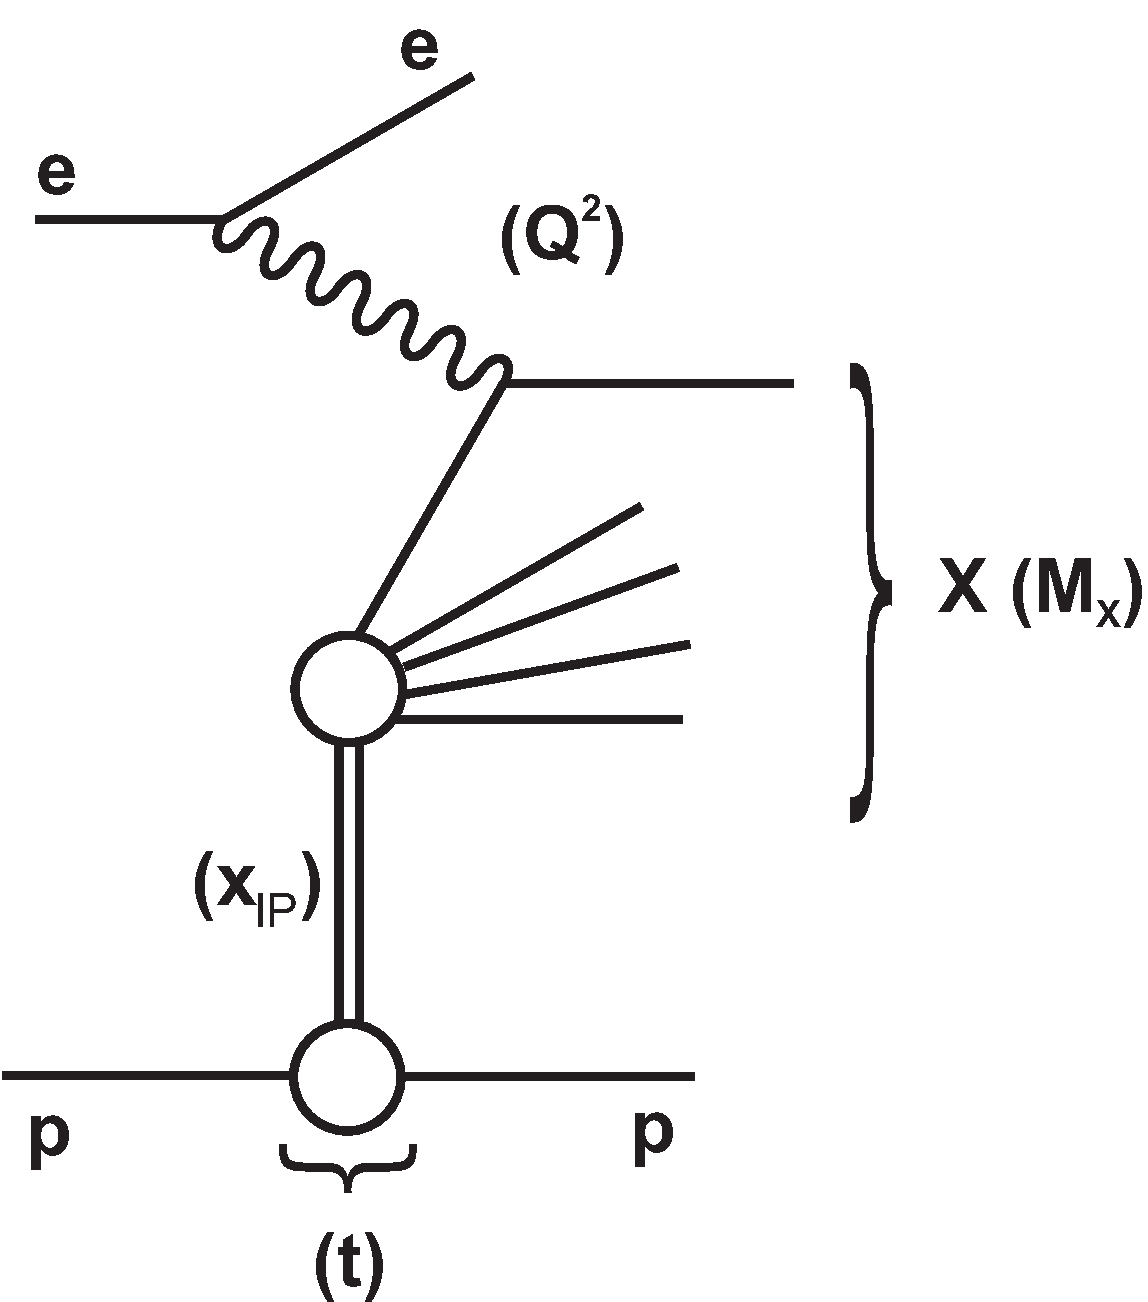
\includegraphics[width=0.5\linewidth]{figures/diffraction.pdf}
\end{center}
\label{fig:diff}
\end{figure}

 In addition to $x$, $Q^2$ and the squared four-momentum transfer $t$
(the undetected momentum transfer to the proton system),
the mass $M_X$ of the diffractively produced final state provides
 a further degree of freedom. In practice, the variable $M_X$ is often replaced by $\beta$,
\begin{equation}
\beta=\frac{Q^2}{M_X^2+Q^2-t}.
\end{equation}

In models based on a factorisable pomeron, $\beta$ may be viewed as the fraction of the
pomeron longitudinal momentum which is carried by the struck parton, $x=\beta\Pom$.
%The diffractive parton distribution functions (DPDFs) are interpreted as probabilities for 
%finding a parton with a small fraction of the proton momentum $x=\beta\Pom$

\subsubsection {Cross-section}

The diffractive structure functions can be expressed as convolutions of the
calculable coefficient functions with diffractive quark and gluon distribution functions,
 which in general depend on all of $x$, $Q^2$, $\beta$, $t$.
\begin{equation}
  \frac{d\sigma}{d\beta\,dQ^2d\xi\,dt}
=
  \frac{2\pi\alpha^2}{\beta Q^4}\,
    \left( 1 +  (1-y)^2 \right) \ensuremath{\overline\sigma}^{D(4)}(\beta,Q^2,\xi,t)
\label{Dxs}
\end{equation}
where the ``reduced cross-section'' , $\overline\sigma$, is defined as
\begin{equation}
\overline\sigma^{D(4)}
 = F_2^{D(4)} - \frac{y^2}{1 +  (1-y)^2}\, F_L^{D(4)}
 = F_T^{D(4)} + \frac{2(1-y)}{1 +  (1-y)^2}\, F_L^{D(4)}
\label{eq:sigred}
\end{equation}
The dimension of $F_k^{D(4)}(\beta,Q^2,\xi,t)$
is $GeV^{-2}$ and thus the quantities integrated over $t$.
\begin{equation}
F_k^{D(3)}(\beta,Q^2,\xi)
\equiv
\int_{t_{\rm min}}^{t_{\rm max}} dt
F_k^{D(4)}(\beta,Q^2,\xi,t)
\end{equation}
are dimensionless. Maximum kinematically allowed value of $t$ reads as
\begin{equation}
t_{\rm MAX} 
=
-\frac{\xi^2 m_p^2 + p_\perp^2}{1-\xi}
\approx 
-\frac{\xi^2}{1-\xi} m_p^2
\end{equation}
where $m_p$ is the proton mass.
As $x = \xi\beta$ we can normalize to the standard DIS formula
\begin{equation}
\frac{d\sigma}{d\beta\,dQ^2\,d\xi\,dt} =
  \frac{2\pi\alpha^2}{x\, Q^4}\,
    \left( 1 +  (1-y)^2 \right) \xi\ensuremath{\overline\sigma}^{D(4)}(\beta,Q^2,\xi,t)
\end{equation}
which upon integration over $t$ reads
\begin{equation}
\label{Dxs3}
  \frac{d\sigma}{d\beta\,dQ^2\,d\xi}
=  
  \frac{2\pi\alpha^2}{x Q^4}\,
    \left( 1 +  (1-y)^2 \right) \,\xi\ensuremath{\overline\sigma}^{D(3)}(\beta,Q^2,\xi).
\end{equation}
%The H1 and ZEUS data files typically contain $\xi\ensuremath{\overline\sigma}^{D(3)}$.

%==========================================
\subsubsection {Regge factorization}
For a  better description of data, a contribution from a secondary Reggeon, $\Reg$, is included, hence
\begin{equation}
F_k^{D(4)}(\beta,Q^2,\xi,t) = 
\sum_{\mathcal{X} =\Pom,\Reg}
\phi_\mathcal{X}(\xi,t)\, F^\mathcal{X}_k(\beta,Q^2)
\end{equation}
or
\begin{equation}
\label{eq:FD3}
F_k^{D(3)}(\beta,Q^2,\xi) = 
\sum_{\mathcal{X} =\Pom,\Reg}
\Phi_\mathcal{X}(\xi)\, F^\mathcal{X}_k(\beta,Q^2)
\end{equation}
where
\begin{equation}
\label{eq:intFlux}
\Phi_{\mathcal{X}}(\xi) =
\int\limits_{t_{\rm min}}^{t_{\rm max}} dt\, \phi_\mathcal{X}(\xi,t)
\,.
\end{equation}
Parametrization of the fluxes follows
\begin{subequations}
\label{eq:flux}
\begin{equation}
\phi_\mathcal{X}(\xi,t) = 
\frac {A_\mathcal{X}\, e^{b_\mathcal{X} t}} {\xi^{2\alpha_\mathcal{X}(t) -1}}
\end{equation}
where
\begin{equation}
\alpha_\mathcal{X}(t) = \alpha_\mathcal{X}(0) + \alpha_\mathcal{X}' t
\,.
\end{equation}
\end{subequations}
$F^\Reg_k(\beta,Q^2)$ are taken as those of the pion.
%  with the normalization factor being absorbed in $\phi_\Reg(\xi,t)$.

%\newcommand\Version{2.01.02}
\newif\ifFullVer\FullVertrue
\FullVerfalse

% \texorpdfstring

\renewcommand\topfraction{0.5}
\renewcommand\bottomfraction{0.5}
\renewcommand\textfraction{0.5}
\renewcommand\floatpagefraction{0.5}

\makeatletter
\def\comsp{\@ifnextchar,\relax{\@ifnextchar\ \relax{\@ifnextchar:\relax{\@ifnextchar.\relax\ }}}}
\makeatother
\DeclareRobustCommand{\ie}{{\it i.e.}\comsp}
\DeclareRobustCommand{\eg}{{\it e.g.}\comsp}
\DeclareRobustCommand{\cf}{{\it cf.}\comsp}
\DeclareRobustCommand{\etal}{{\it et al.}\comsp}
\DeclareRobustCommand\bs{\ensuremath{\backslash}}
\newcommand\ssp{\ifmmode\relax\else\comsp\fi}

%\newcommand\Eq[1]{Eq.~(\ref{#1})}
\newcommand\Eq[1]{(\ref{#1})}
\newcommand\Fig[1]{Fig.~\ref{#1}}
\DeclareRobustCommand\NF{\ensuremath{N_{\rm f}}\ssp}
% \DeclareRobustCommand\NC{\ensuremath{N_{\rm c}}\ssp}
\DeclareRobustCommand\GeV{\ensuremath{{\rm GeV}}\ssp}
% \DeclareRobustCommand\Vstat{\ensuremath{V^{\rm (stat)}}\ssp}
% \DeclareRobustCommand\Vsys{\ensuremath{V^{\rm (sys)}}\ssp}
\DeclareRobustCommand\FL{\ensuremath{F_{\mathrm{L}}}\ssp}
\DeclareRobustCommand\FT{\ensuremath{F_{\mathrm{T}}}\ssp}
\newcommand\AP {{\cal P}}

\def \beq{\begin{equation}}
\def \eeq{\end{equation}}
\def \beqa{\begin{eqnarray}}
\def \eeqa{\end{eqnarray}}
\def \beqal{\begin{subequations}\begin{eqnarray}}
\def \eeqal{\end{eqnarray}\end{subequations}}

\let\optspace=\ssp
% \newcommand{\xh}{\hat x}
\DeclareRobustCommand{\as}[1]{\ensuremath{\alpha_{\rm s}(#1^2)}\optspace}
\newcommand{\asotp}{\ensuremath{\frac{\alpha_{\rm s}}{2\pi}}\optspace}
\newcommand{\Sgl}[1]{\ensuremath{\tilde f_{#1+}}\optspace}
\newcommand{\Pom}{{I\!P}}
\newcommand{\Reg}{{I\!R}}
% \newcommand{\xP}{x_\Pom}
\newcommand{\xP}{\xi}
\newcommand\sigRed{\ensuremath{\overline\sigma}}
\newcommand\DX{\ensuremath{\mathcal{X}}}

%\parindent=0pt
%\parskip=4pt

%\graphicspath{{figs/}}

%==========================================
\subsubsection {Cross-section}

\beq
  \frac{d\sigma}{d\beta\,dQ^2\,d\xP\,dt}
=
  \frac{2\pi\alpha^2}{\beta Q^4}\,
    \left( 1 +  (1-y)^2 \right) \sigRed^{D(4)}(\beta,Q^2,\xP,t)
\label{Dxs}
\eeq
where the `reduced cross-section', \sigRed, is defined as
\beq
\label{eq:sigred}
\sigRed
 = F_2 - \frac{y^2}{1 +  (1-y)^2}\, \FL
 = \FT + \frac{2(1-y)}{1 +  (1-y)^2}\, \FL
\eeq
Nb. $\xi$ is denoted by $x_\Pom$ in the H1 and ZEUS papers.

The dimension of 
\(
F_k^{D(4)}(\beta,Q^2,\xP,t)\)
is $\GeV^{-2}$
and
thus the quantities integrated over $t$
\beq
F_k^{D(3)}(\beta,Q^2,\xP)
\equiv
\int_{t_{\rm min}}^{t_{\rm max}} dt
F_k^{D(4)}(\beta,Q^2,\xP,t)
\eeq
are dimensionless.

Maximum kinematically allowed value of $t$ reads
\begin{equation}
t_{\rm MAX} 
=
-\frac{\xP^2 m_p^2 + p_\perp^2}{1-\xP}
\approx 
-\frac{\xP^2}{1-\xP} m_p^2
\end{equation}
where $m_p$ is the proton mass.

As $x = \xP\beta$ we can normalize to the standard DIS formula
\begin{equation}
\frac{d\sigma}{d\beta\,dQ^2\,d\xP\,dt} =
  \frac{2\pi\alpha^2}{x\, Q^4}\,
    \left( 1 +  (1-y)^2 \right) \xP\sigRed^{D(4)}(\beta,Q^2,\xP,t)
\end{equation}
which upon integration over $t$ reads
\begin{equation}
\label{Dxs3}
  \frac{d\sigma}{d\beta\,dQ^2\,d\xP}
=  
  \frac{2\pi\alpha^2}{x Q^4}\,
    \left( 1 +  (1-y)^2 \right) \,\xi\sigRed^{D(3)}(\beta,Q^2,\xP)
\end{equation}


The H1 and ZEUS data files typically contain $\xP\sigRed^{D(3)}$.

%==========================================
\subsubsection {Regge factorization}

For better data description we include a contribution from a secondary Reggeon, $\Reg$,
\beq
F_k^{D(4)}(\beta,Q^2,\xP,t) = 
\sum_{\mathcal{X} =\Pom,\Reg}
\phi_\mathcal{X}(\xP,t)\, F^\mathcal{X}_k(\beta,Q^2)
\eeq

or
\beq
\label{eq:FD3}
F_k^{D(3)}(\beta,Q^2,\xP) = 
\sum_{\mathcal{X} =\Pom,\Reg}
\Phi_\mathcal{X}(\xP)\, F^\mathcal{X}_k(\beta,Q^2)
\eeq
where
\begin{equation}
\label{eq:intFlux}
\Phi_{\mathcal{X}}(\xP) =
\int\limits_{t_{\rm min}}^{t_{\rm max}} dt\, \phi_\mathcal{X}(\xP,t)
\,.
\end{equation}

Parametrization of the fluxes
\begin{subequations}
\label{eq:flux}
\begin{equation}
\phi_\mathcal{X}(\xP,t) = 
\frac {A_\mathcal{X}\, e^{b_\mathcal{X} t}} {\xP^{2\alpha_\mathcal{X}(t) -1}}
\end{equation}
where
\begin{equation}
\alpha_\mathcal{X}(t) = \alpha_\mathcal{X}(0) + \alpha_\mathcal{X}' t
\,.
\end{equation}
\end{subequations}

$F^\Reg_k(\beta,Q^2)$ are taken as those of the pion.
%  with the normalization factor being absorbed in $\phi_\Reg(\xP,t)$.


%==========================================
\subsubsection {Pomeron parametrization}

The Pomeron is parametrized at the initial
$Q_0^2$ in terms of two singlet distributions,
$f_{g}$ and $f_{+}$.
\begin{subequations}
\label{singlet}
\begin{eqnarray}
\frac{d}{dt}f_{+} &=&
\asotp\left[
\AP_{\rm FF} f_{+} +\AP_{\rm FG}f_g
\right]
\\
\frac{d}{dt}f_{g} &=&
\asotp\left[
\AP_{\rm GF} f_{+} +\AP_{\rm GG}f_g
\right]
\end{eqnarray}
\end{subequations}

As $\Pom$ is neutral, $f_{q} = f_{\bar q}$ for each flavour $q$.
Assuming that all light quark PDFs are equal
\begin{equation}
f_d = f_u = f_s
\,,
\end{equation}
we have
\begin{subequations}
\label{eq:pm}
\begin{eqnarray}
f_{q-} &\equiv& 0
\\
f_{q+} &\equiv& 2 f_q
\end{eqnarray}
\end{subequations}

At \NF = 3
\begin{equation}
\label{eq:fq3}
f_{q+} = f_{+}/3,\; q = d,u,s
\,.
\end{equation}
\ifFullVer
\ie
\begin{equation}
\Sgl q = 0,\; q = d,u,s
\,,
\end{equation}
where
\begin{equation}
\Sgl q \equiv f_{q+} - \frac{1}{\NF}f_{+}
\,.
\end{equation}
\fi

This gives all PDFs for the FFNS, while for VFNS 
$f_{h+}, h=c,b,t$ are generated dynamically above the respective
transition scales $Q_h^2$.
Hence at \NF > 3 the singlet has contributions from the heavy quarks
and we get non-trivial nonsinglet distributions $\Sgl{h}$ satisfying
\begin{equation}
\label{eq:nsevol}
\frac{d}{dt}\Sgl h = \asotp\, \AP_{(+)} \Sgl h
\end{equation}

%\subsection {Parametrization at \texorpdfstring{$Q_0^2$}{Q0}}
%\subsubsection {Parametrization at {$Q_0^2$}}
{\bf Parametrization at {$Q_0^2$}} \\
%-----------------------------------------------------------
\label{sec:Par}

Full PDFs are given in analogy to \Eq{eq:FD3}
\begin{equation}
f_k^{D(3)}(\beta,Q^2,\xP) =
\hat\Phi_\Pom(\xP)\, f^\Pom_k(\beta,Q^2)
+
\Phi_\Reg(\xP)\, f^\Reg_k(\beta,Q^2)
\end{equation}
where $\hat\Phi_\Pom \equiv \Phi_\Pom/A_\Pom$,
with the fluxes given by \Eq{eq:intFlux} and \Eq{eq:flux}.

The Pomeron PDFs (omitting superscript $\Pom$) are parametrized as
\def\Cini#1#2{A^{(#1)}_#2}
\begin{equation}
\label{eq:fP0}
f_N = \Cini N1  x^{\Cini N2} (1-x)^{\Cini N3}
%   \left(1 + \Cini N4 x \right)
  \; \exp\left(-\frac{d}{1.00001-x}\right)
\,,
\end{equation}
where the `dumping factor' $d$ is taken as 0.01 or 0.001.
$N =$ G for gluon or S for `singlet': $f_{\rm S} \equiv f_+(\NF=3)$,
\cf \Eq{eq:fq3}.

% The Reggeon PDFs $f^\Reg_k$ are taken from pion.

%\subsubsection {HERAFitter parameters}
{\bf HERAFitter parameters} \\
%-----------------------------------------------------------
\label{sec:HFitterPar}

% minuit.in.txt
% ExtraMinimisationParameters

\begin{tabular}{l|l|l}
Parameter & HERAFitter name & input file\\
% \hline
$\Cini {\mathrm G}1$ & Ag & minuit.in.txt \\
$\Cini {\mathrm G}2$ & Bg & minuit.in.txt \\
$\Cini {\mathrm G}3$ & Cg & minuit.in.txt \\
$\Cini {\mathrm S}1$ & Auv & minuit.in.txt \\
$\Cini {\mathrm S}2$ & Buv & minuit.in.txt \\
$\Cini {\mathrm S}3$ & Cuv & minuit.in.txt \\
$\alpha_\Pom(0)$ & Pomeron\_a0 & steering.txt \\
$A_\Reg$ & Reggeon\_factor & steering.txt \\
$\alpha_\Reg(0)$ & Reggeon\_a0 & steering.txt \\
\end{tabular}




        

